% ------------------------------------------------------------------------------------
% ------------------------------ GESTION DE USUARIOS ---------------------------------
% ------------------------------------------------------------------------------------
\clearpage
\section{Gestión de Usuarios}

El usuario  Jefe de División de Innovación Académica  realiza la gestión sobre los siguientes usuarios:
\begin{itemize}
	\item Jefe de Departamento e Innovación Curricular.
	\item Analista.
\end{itemize}
\subsection{Consulta de Usuarios}

El Jefe de División de Innovación Académica  selecciona  la opción \textbf{Gestionar Usuarios} del menú ubicado en la parte izquierda, lo que le muestra la lista de usuarios que tiene a su cargo en la siguiente pantalla:

% Imagen de Consultar usuarios
\begin{figure}[H]
	\centering
	\hypertarget{consultarUs}{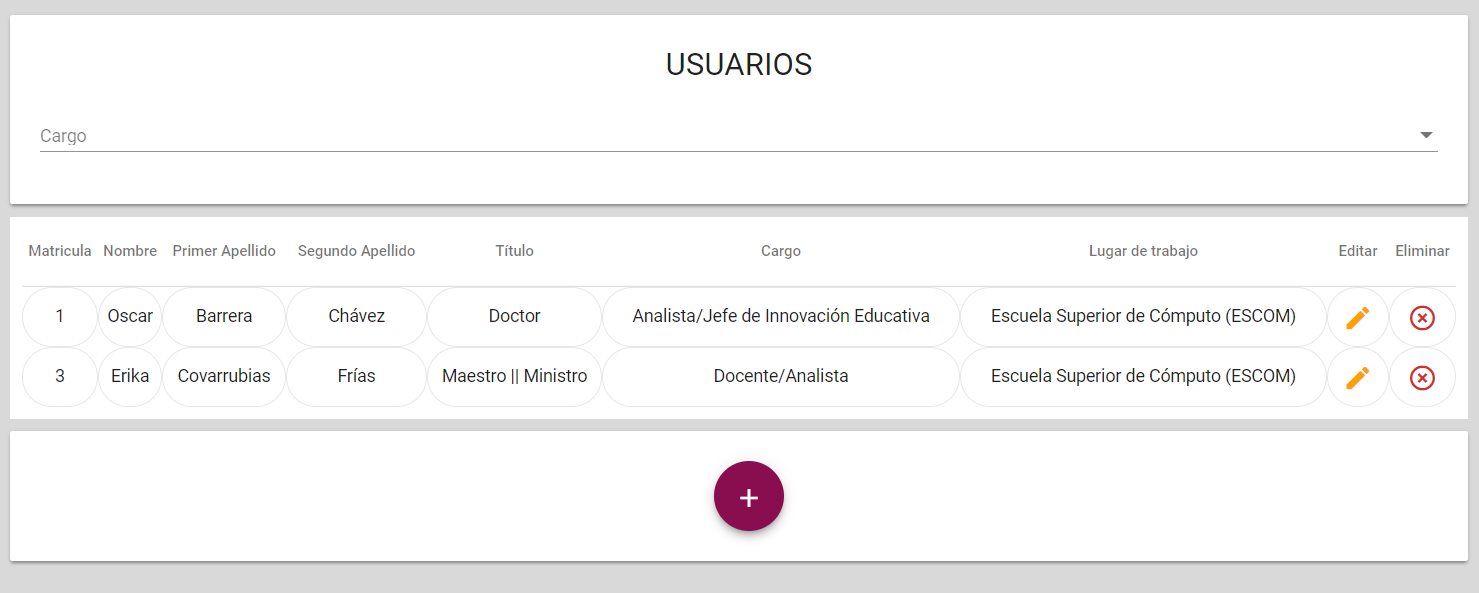
\includegraphics[width=0.6\linewidth]{images/SP5/Consultar-Usuario}}
	\caption{Pantalla para consultar usuarios}
	\label{consultarrh}
\end{figure}

En esa pantalla, aparece de forma predeterminada todos los usuarios que el Jefe de División de Innovación Académica  tiene a su cargo y que están registrados en el sistema hasta el momento. El Jefe de División de Innovación Académica  tiene a su disposición 2 funciones:

\begin{enumerate}
	
	\item   Búsqueda de  usuarios según el cargo que ocupan.
	
	Para esto el Jefe de División de Innovación Académica  solo tiene que seleccionar el cargo que desea consultar en el siguiente componente:
	
	\begin{figure}[H]
		\centering
		\hypertarget{cargo1}{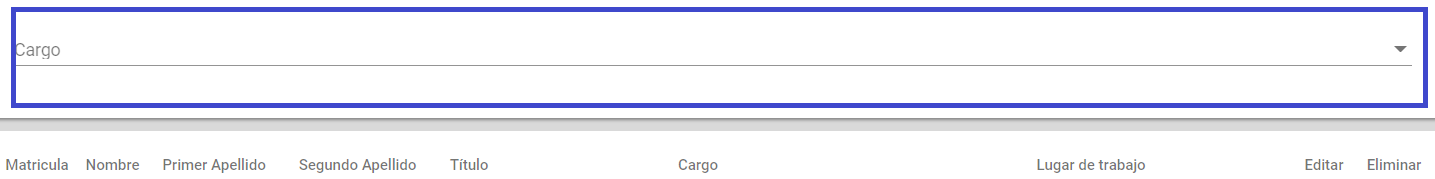
\includegraphics[width=0.7\linewidth]{images/SP5/BtnCargo1}}
		\caption{Selección de Cargo}
		\label{cargo1}
	\end{figure}
	
	Y a continuación el sistema muestra todos los usuarios que tienen el cargo seleccionado.
	
	\newpage
	
	\item Eliminar usuarios.
	
	Para esta última acción, El Jefe de División de Innovación Académica  solo debe dar clic en el botón con el icono de una equis en color rojo que está al lado del usuario que desee eliminar.
	
	\begin{figure}[H]
		\centering
		\hypertarget{eliminar}{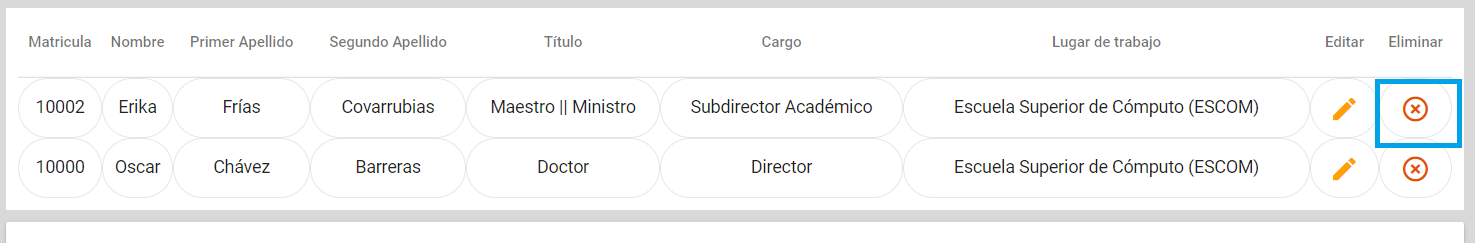
\includegraphics[width=0.7\linewidth]{images/SP5/BtnEliminar}}
		\caption{Botón Eliminar Usuarios}
		\label{eliminar}
	\end{figure}
	
	Al hacer esto, el sistema despliega el siguiente mensaje:
	
	%Imagen del MSG22
	\begin{figure}[H]
		\centering
		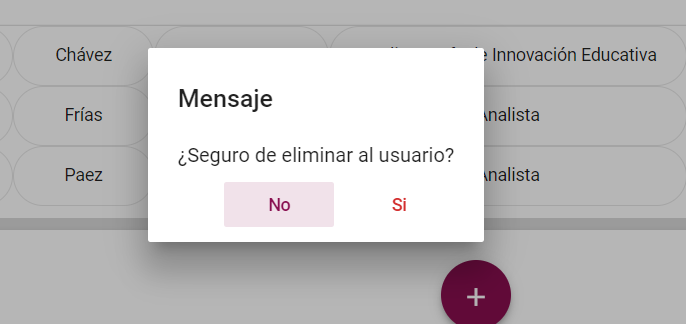
\includegraphics[width=0.4\linewidth]{images/SP5/MSG22}
		\caption{Confirmación de eliminación}
		\label{confirmarE}
		
	\end{figure}
	
	Para confirmar, el Jefe de División de Innovación Académica  debe dar clic en el botón “Sí”, y en ese momento el usuario previamente seleccionado es eliminado del sistema y el Jefe de División de Innovación Académica  permanece en la pantalla \hyperlink{consultarUs}{\textit{Consultar Usuarios}}.
	Para cancelar, el Jefe de División de Innovación Académica  debe dar clic en botón “No”, y en ese momento el mensaje se cierra, el usuario no se elimina, y el Jefe de División de Innovación Académica  permanece en la pantalla de \hyperlink{consultarUs}{\textit{Consultar Usuarios}}.
	
\end{enumerate}

También mediante botones de esta pantalla se puede acceder a las siguientes 2 funciones:

\subsubsection{Editar usuarios}

Para esto, el Jefe de División de Innovación Académica  solo debe dar clic en el botón con el icono de un lápiz amarillo que está al lado del usuario que desee modificar. Al hacer esto el sistema muestra la pantalla  de \hyperlink{editarUs}{\textit{Editar Usuario}}.

\begin{figure}[H]
	\centering
	\hypertarget{editar}{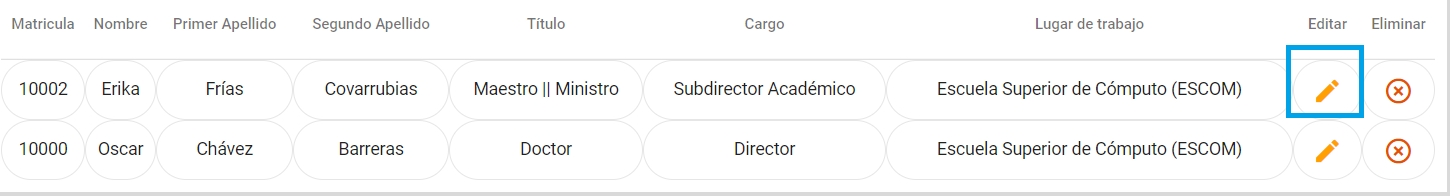
\includegraphics[width=0.7\linewidth]{images/SP5/BtnEditar}}
	\caption{Botón Editar Usuarios}
	\label{editar}
\end{figure}

Para más detalles de editar usuarios vaya a la sección \hyperlink{editar-user}{Edición de Usuarios}.

\subsubsection{Registrar  usuarios}

Para esto el Jefe de División de Innovación Académica  tiene que dar clic en el botón “+” en la parte inferior de la pantalla. Al hacerlo, el sistema  lo redirecciona a la pantalla de \hyperlink{registrarUs}{\textit{Registrar Usuario}}.

\begin{figure}[H]
	\centering
	\hypertarget{add}{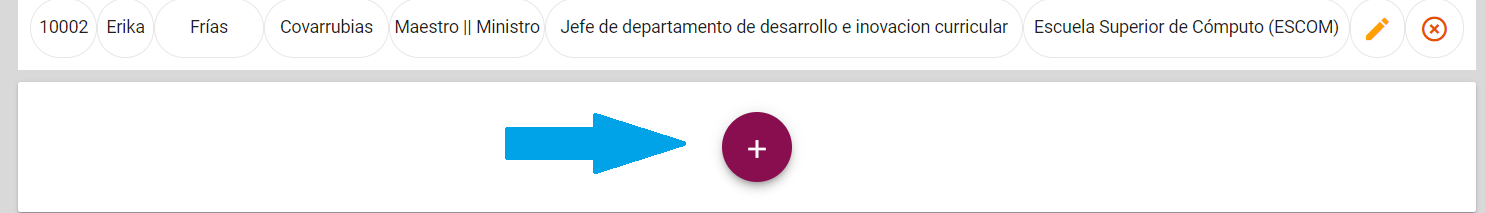
\includegraphics[width=0.7\linewidth]{images/SP5/BtnAgregar}}
	\caption{Botón Agregar Usuarios}
	\label{add}
\end{figure}

Para más detalles de registrar usuarios vaya a la sección \hyperlink{registrar-Us}{Registrar usuario}.

\subsubsection{Posibles errores}
\begin{itemize}
	\item Si el Jefe de División de Innovación Académica   presiona la opción Gestionar Usuarios y no se carga la información de los cargos disponibles para el se presenta el siguiente mensaje:
	
	% Imagen del MSG7
	\begin{figure}[H]
		\centering
		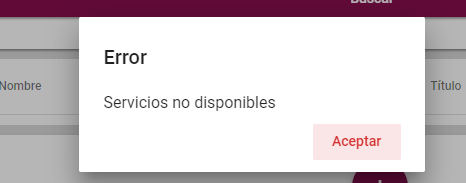
\includegraphics[width=0.4\linewidth]{images/SP5/MSGSN}
		\caption{Servicios no disponibles}
		\label{SND}
		
	\end{figure}
	
	Presiona clic en el botón ''Aceptar'' y  el sistema continua en la pantalla  \hyperlink{consultarUs}{\textit{Consultar Usuarios}} y el Jefe de División de Innovación Académica  tiene que intentarlo  mas tarde.
	
	\item Si en la consulta de usuarios no se encuentra ninguno con el cargo solicitado se presenta el siguiente mensaje:
	% Imagen del MSG21
	\begin{figure}[H]
		\centering
		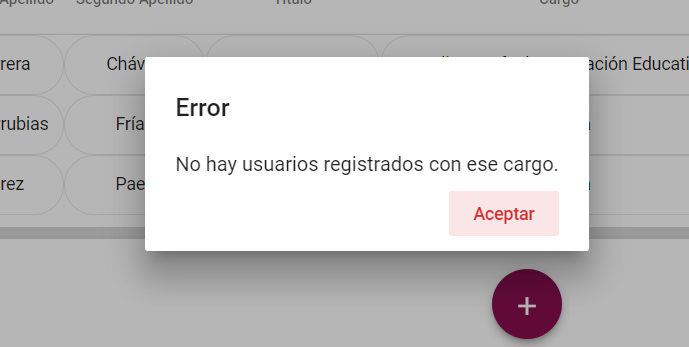
\includegraphics[width=0.4\linewidth]{images/SP5/MSG21}
		\caption{No hay usuarios con ese cargo}
		\label{mensaje21}
	\end{figure}
	
\end{itemize}

% ------------------------------------------------------------------------------------
% ----------------------------- REGISTRAR  USUARIOS ---------------------------------
% ------------------------------------------------------------------------------------

\newpage
\hypertarget{registrarUs}{}
\subsection{Registrar Usuarios}
Si el Jefe de División de Innovación Académica   en la pantalla de \hyperlink{consultarUs}{\textit{Consultar Usuarios}} da clic en el botón ''+'', aparece la siguiente pantalla:

\begin{figure}[H]
	\centering
	\hypertarget{registrar-Us}{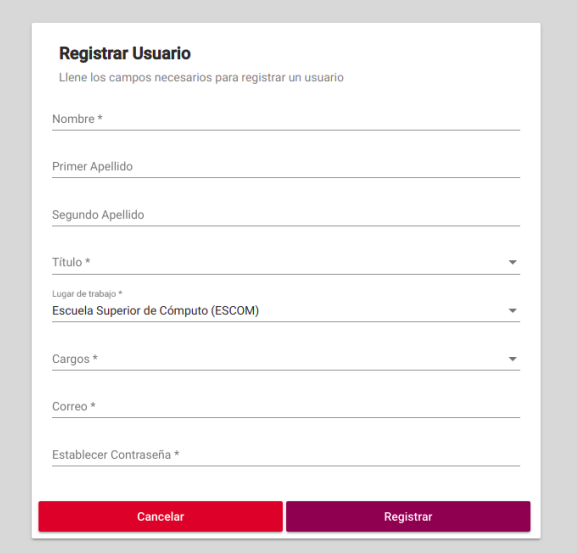
\includegraphics[width=0.7\linewidth]{images/SP5/Registro-Usuario-vacio}}
	\caption{Pantalla para registrar usuarios}
	\label{registrarrh}
\end{figure}

El Jefe de División de Innovación Académica  tiene que ingresar la información correspondiente del nuevo usuario en el formulario. Un ejemplo del llenado  es el siguiente:

\begin{figure}[H]
	\centering
	\hypertarget{ejreg}{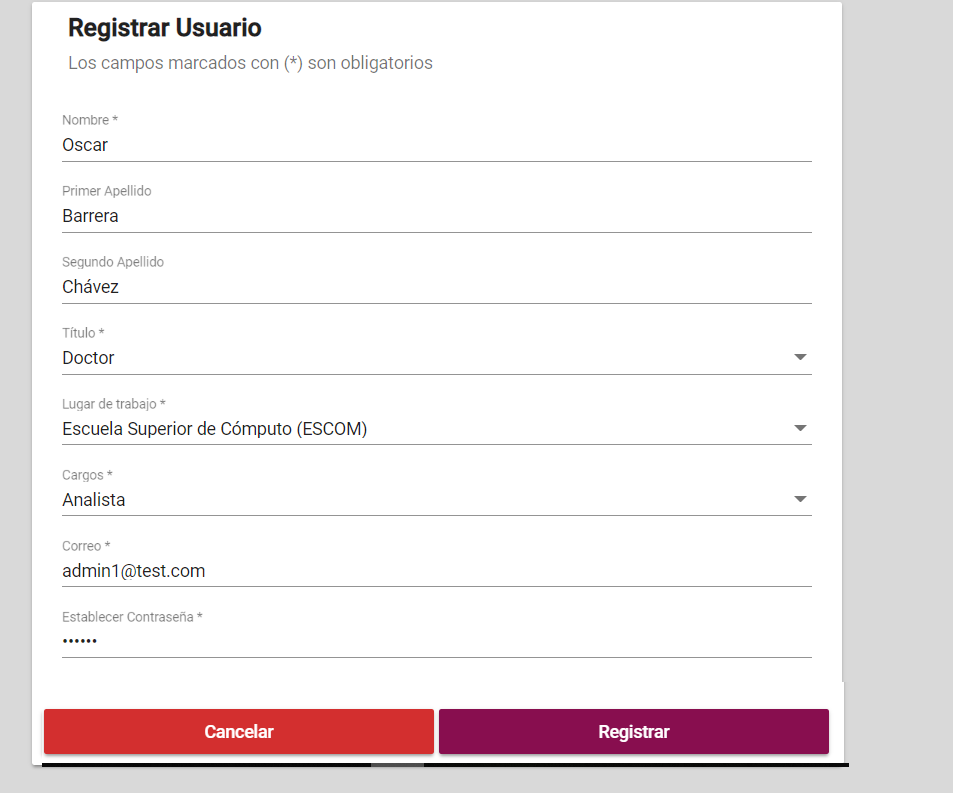
\includegraphics[width=0.7\linewidth]{images/SP5/Registro-Usuario-UA}}
	\caption{Ejemplo de llenado para agregar un nuevo Usuario}
	\label{ejreg}
\end{figure}

\newpage
Si el Jefe de División de Innovación Académica  presiona el botón de “Cancelar”:

\begin{figure}[H]
	\centering
	\hypertarget{cancel1}{
\includegraphics[width=0.7\linewidth]{images/SP5/BtnCancelar1}}
	\caption{Botón ''Cancelar''}
	\label{cancel1}
\end{figure}

El sistema muestra el siguiente mensaje:

%Imagen MSG29

\begin{figure}[H]
	\centering
	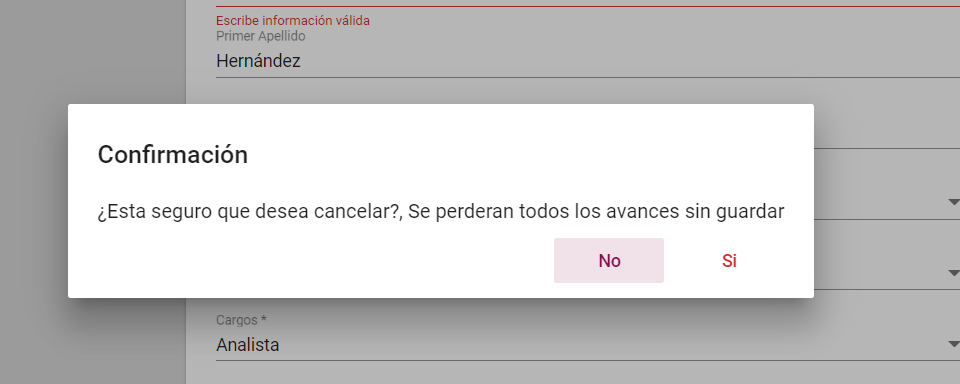
\includegraphics[width=0.4\linewidth]{images/SP5/MSG29}
	\caption{Cancelar Accion}
	\label{mensaje29}
\end{figure}

Para confirmar, el Jefe de División de Innovación Académica  tiene que dar clic en el botón “Sí”, el usuario no es registrado y regresa a la pantalla de \hyperlink{consultarUs}{\textit{Consultar Usuarios}}.

Para que el registro continué , el Jefe de División de Innovación Académica  tiene que  dar clic el botón “No”, el mensaje se  cierra  y el continúa en el formulario para terminar el registro.

Si el Jefe de División de Innovación Académica  considera que los datos son correctos y están completos, debe de dar clic en el botón “Registrar”.

\begin{figure}[H]
	\centering
	\hypertarget{btnreg}{
\includegraphics[width=0.7\linewidth]{images/SP5/BtnRegistrar}}
	\caption{Botón ''Registrar''}
	\label{btnreg}
\end{figure}

Si no se presentan errores el sistema muestra el mensaje:

% Imagen MSG5

\begin{figure}[H]
	\centering
	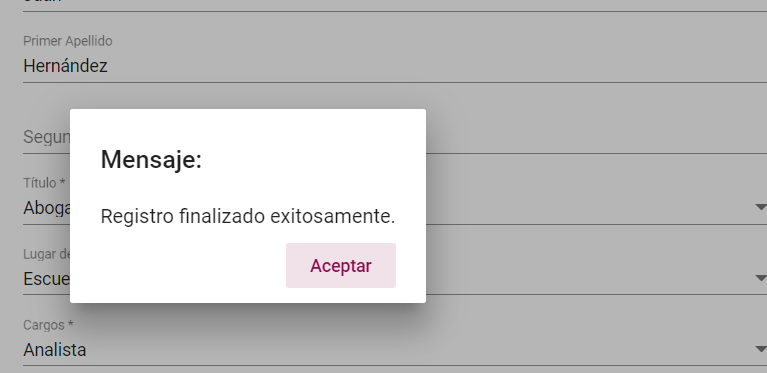
\includegraphics[width=0.4\linewidth]{images/SP5/MSG5}
	\caption{Registro exitoso}
	\label{mensaje5}
	
\end{figure}

Si el Jefe de División de Innovación Académica   da clic en el botón “Aceptar”, el sistema muestra la pantalla de  \hyperlink{consultarUs}{\textit{Consultar Usuarios}}.

\subsubsection{Posibles errores}

\begin{itemize}
	\item Problemas con la conexión o el sistema
	
	Si cuando el Jefe de División de Innovación Académica  accede a la pantalla de \hyperlink{registrarUs}{\textit{Registrar Usuario}} o al intenta registrar un usuario , aparece el siguiente mensaje:
	%Imagen MSG7 Y MSG25
	
	\begin{figure}[H]
		\centering
		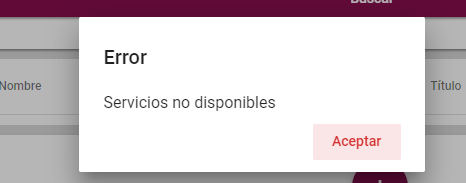
\includegraphics[width=0.4\linewidth]{images/SP5/MSGSN}
		\caption{Servicios no disponibles}
		\label{SND}
		
	\end{figure}
	
	Significa que existió un error de conexión o del sistema. El Jefe de División de Innovación Académica  da clic en el botón ''Aceptar'' y el sistema lo redirecciona  a la pantalla de \hyperlink{consultarUs}{\textit{Consultar Usuarios}}. El Jefe de División de Innovación Académica  debe esperar a que la página este disponible para intentar acceder nuevamente.
	
	\item Campos vacíos al momento de agregar un nuevo usuario
	
	Si el Jefe de División de Innovación Académica  deja en blanco algún campo o campos del formulario, y posteriormente da clic en el botón ''Registrar'', el sistema muestra el siguiente mensaje debajo del campo o campos :
	%Imagen MSG44
	
	\begin{figure}[H]
		\centering
		
\includegraphics[width=0.4\linewidth]{images/SP5/MSG44}
		\caption{Campos vacíos}
		\label{mensaje44}
	\end{figure}
	
	El sistema regresa al formulario, en donde el Jefe de División de Innovación Académica  debe llenar el o los campos que dejo vacíos.
	
	\item El correo ingresado ya existe
	
	Si cuando el Jefe de División de Innovación Académica  da clic en el botón ''Registrar'' aparece el siguiente mensaje:
	%Imagen MSG36
	
	\begin{figure}[H]
		\centering
		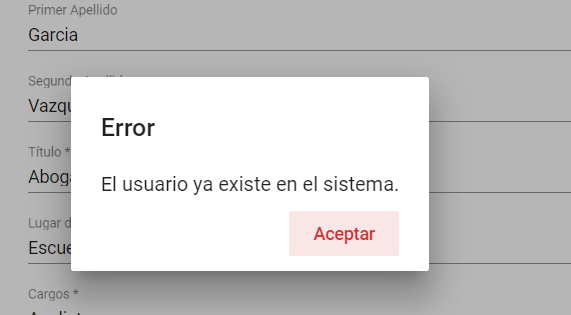
\includegraphics[width=0.4\linewidth]{images/SP5/MSG36}
		\caption{El usuario ya existe}
		\label{mensaje36}
		
	\end{figure}
	
	Significa que el usuario ya se encuentra registrado en el sistema, por lo que éste impide que se vuelva a agregar nuevamente. Si el Jefe de División de Innovación Académica  da clic en botón ''Aceptar'', el mensaje se cierra y el sistema regresa al formulario. Ahí el Jefe de División de Innovación Académica   puede hacer dos acciones: verifica que el correo sea uno no registrado previamente e intenta agregar al usuario nuevamente, o abandona la pantalla de \hyperlink{registrarUs}{\textit{Registrar Usuarios}} y va a otras partes del sistema.
	
	\item Los campos ingresados no son válidos
	
	Si al momento de dar clic en el botón ''Registrar'' aparece el siguiente mensaje:
	%Imagen MSG35
	% Imagen del MSG35
	\begin{figure}[H]
		\centering
		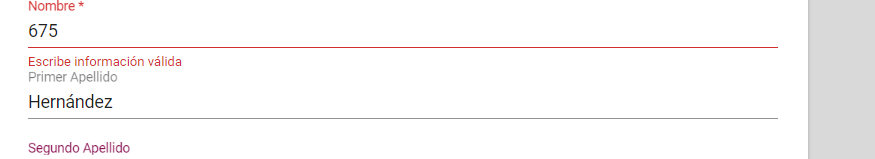
\includegraphics[width=0.4\linewidth]{images/SP5/MSG35}
		\caption{Campos incorrectos}
		\label{mensaje35}
		
	\end{figure}
	
	Significa que la composición de los datos ingresados en el formulario no es la correcta. El Jefe de División de Innovación Académica  debe tener en cuenta lo siguiente:
	
	\begin{itemize}
		\item El nombre y apellidos debe iniciar con mayúscula, se puede poner más de uno por campo en caso de 2 nombres o apellidos compuestos.
		\item El Jefe de División de Innovación Académica  altera la información de los selectores de cargo o zona de trabajo.
		\item La contraseña no acepta acentos, espacios o caracteres especiales.
	\end{itemize}
	
\end{itemize}

% ------------------------------------------------------------------------------------
% ------------------------------ EDICION DE USUARIOS ---------------------------------
% ------------------------------------------------------------------------------------
\newpage

\hypertarget{editar-user}{}
\subsection{Edición de Usuarios}
Si el Jefe de División de Innovación Académica  en la pantalla de \hyperlink{consultarUs}{\textit{Consultar Usuarios}} da clic en el botón con el icono de un lápiz amarillo de un usuario, aparece la siguiente pantalla:

\begin{figure}[H]
	\centering
	\hypertarget{editarUs}{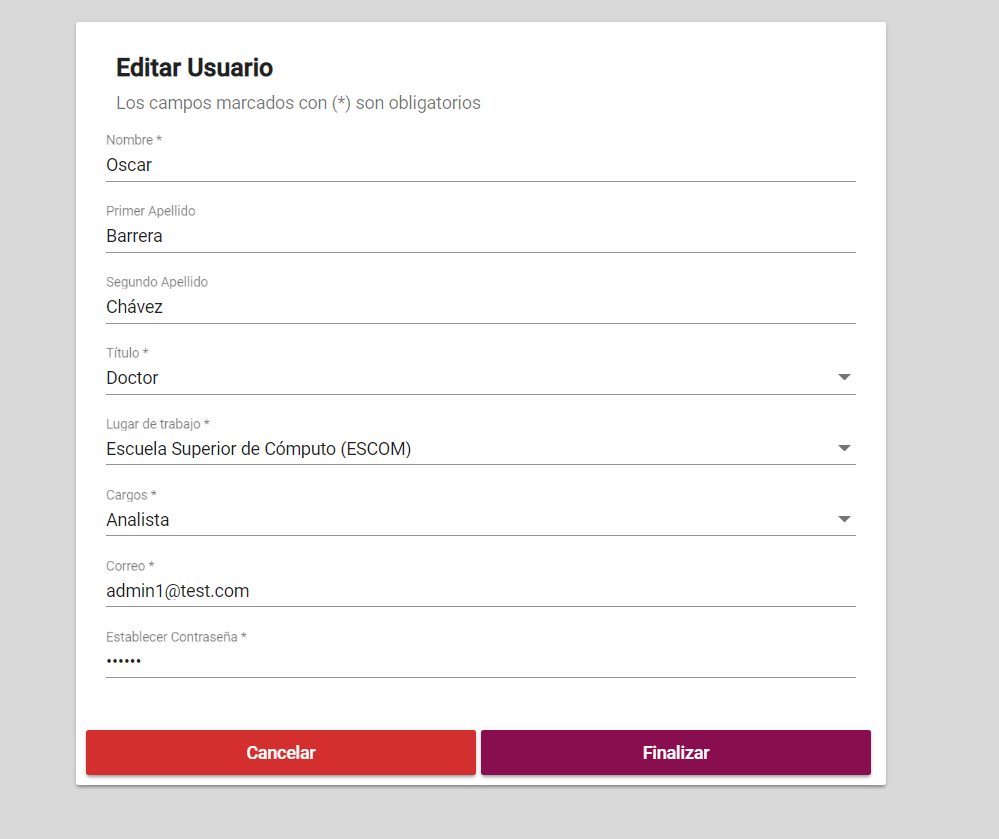
\includegraphics[width=0.6\linewidth]{images/SP5/Editar-Usuario}}
	\caption{Pantalla para la edición de Usuarios}
	\label{editarrh}
\end{figure}

En esta pantalla se cargan los datos del usuario correspondiente por el lápiz amarillo seleccionado en la pantalla de \hyperlink{consultarUs}{\textit{Consultar Usuarios}} y se llena el formulario.

A continuación, el Jefe de División de Innovación Académica  pude modificar todos los campos del usuario.

Si el Jefe de División de Innovación Académica  presiona el botón de “Cancelar”:

\begin{figure}[H]
	\centering
	\hypertarget{cancel2}{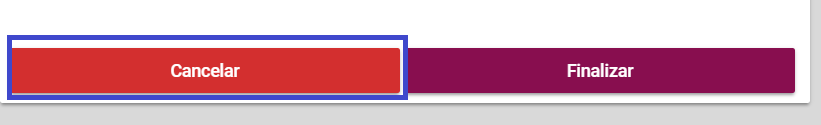
\includegraphics[width=0.7\linewidth]{images/SP5/BtnCancelar2}}
	\caption{Botón ''Cancelar''}
	\label{cancel2}
\end{figure}

El sistema muestra el siguiente mensaje:
%Imagen MSG29
\clearpage
\begin{figure}[H]
	\centering
	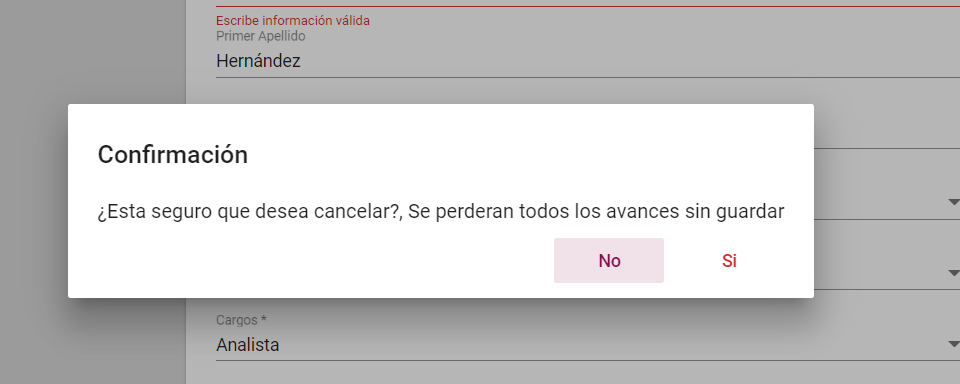
\includegraphics[width=0.4\linewidth]{images/SP5/MSG29}
	\caption{Cancelar cambios}
	\label{mensaje29}
	
\end{figure}

Para confirmar, el Jefe de División de Innovación Académica  da clic en el botón “Sí” y los datos del usuario no son modificados, el Jefe de División de Innovación Académica  regresa a la pantalla \hyperlink{consultarUs}{\textit{Consultar Usuarios}}

Para continuar con la modificación, el Jefe de División de Innovación Académica   da clic el botón “No”, el mensaje se cierra y el Jefe de División de Innovación Académica  continúa en el formulario, donde finaliza la modificación.

Cuando el Jefe de División de Innovación Académica  considere que los datos son correctos y están completos, da clic en el botón “Finalizar”.
\begin{figure}[H]
	\centering
	\hypertarget{btnfin}{
\includegraphics[width=0.7\linewidth]{images/SP5/BtnFinalizar}}
	\caption{Botón ''Finalizar''}
	\label{btnfin}
\end{figure}

Si no se presentan errores el sistema muestra el mensaje:
%Imagen MSG31

\begin{figure}[H]
	\centering
	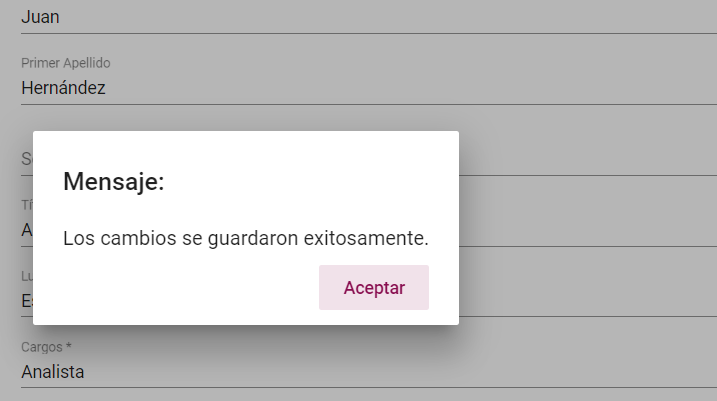
\includegraphics[width=0.4\linewidth]{images/SP5/MSG31}
	\caption{Cambios guardados}
	\label{mensaje31}
	
\end{figure}

Al dar clic en el botón “Aceptar”, el sistema muestra la pantalla de \hyperlink{consultarUs}{\textit{Consultar Usuarios}}.

\subsubsection{Posibles errores}
\begin{itemize}
	\item Problemas con la conexión o el sistema
	
	Si cuando el Jefe de División de Innovación Académica  accede la pantalla de \hyperlink{editarUs}{\textit{Editar Usuario}} o intenta modificar un usuario, aparece el siguiente mensaje:
	\clearpage
	\begin{figure}[H]
		\centering
		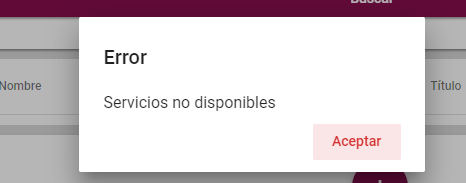
\includegraphics[width=0.4\linewidth]{images/SP5/MSGSN}
		\caption{Servicios no disponibles}
		
	\end{figure}
	
	
	Significa que existe un error de conexión o del sistema. El Jefe de División de Innovación Académica  da clic en el botón ''Aceptar'', el sistema lo redirecciona  a la pantalla de \hyperlink{consultarUs}{\textit{Consultar Usuarios}}. Ahí  espera a que la página este disponible para intentar acceder nuevamente.
	
	\item Campos vacíos al momento de modificar al usuario
	
	Si el Jefe de División de Innovación Académica  deja en blanco algún campo o campos del formulario, y posteriormente da clic en el botón ''Finalizar'', el sistema muestra el siguiente mensaje debajo del campo o campos vacíos:
	%Imagen MSG3X
	
	\begin{figure}[H]
		\centering
		
\includegraphics[width=0.4\linewidth]{images/SP5/MSG44}
		\caption{Campos vacíos}
		\label{mensaje44}
		
	\end{figure}
	
	El sistema regresa  al formulario, en donde el Jefe de División de Innovación Académica  llena el o los campos que dejo vacíos.
	\item El correo ingresado ya existe
	
	Si al momento de dar clic en el botón ''Finalizar'' aparece el siguiente mensaje:
	%Imagen MSG36
	
	\begin{figure}[H]
		\centering
		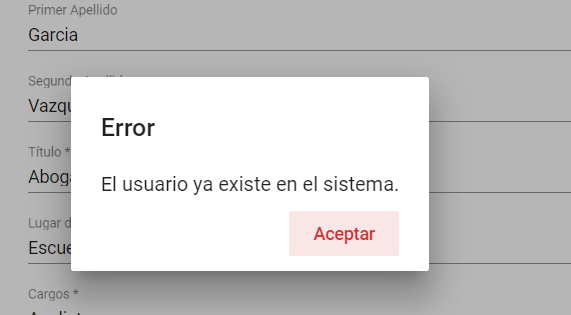
\includegraphics[width=0.4\linewidth]{images/SP5/MSG36}
		\caption{El usuario ya existe}
		\label{mensaje36}
		
	\end{figure}
	
	Significa que el usuario ya se encuentra registrado en el sistema, por lo que éste impide que se vuelva a agregar nuevamente. El Jefe de División de Innovación Académica  da clic en el botón ''Aceptar'', el mensaje se cierra y el sistema regresa al formulario. Ahí el Jefe de División de Innovación Académica  puede hacer dos acciones: verifica que el correo sea uno no registrado previamente y agrega al Usuario nuevamente, o abandona la pantalla de \hyperlink{registrarUs}{\textit{Registrar Usuarios}} y va a otras partes del sistema.
	
	\item Los campos ingresados no son válidos
	
	Si al momento de dar clic en el botón ''Finalizar'' aparece el siguiente mensaje:
	
	\begin{figure}[H]
		\centering
		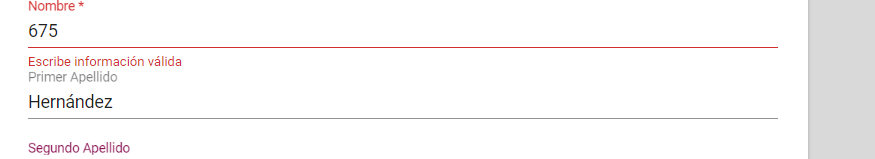
\includegraphics[width=0.4\linewidth]{images/SP5/MSG35}
		\caption{Campos incorrectos}
		\label{mensaje35}
		
	\end{figure}
	
	
	Significa que la composición de los datos ingresados en el formulario no es la correcta. Tenga en cuenta lo siguiente:
	
	\begin{itemize}
		\item El nombre y apellidos debe iniciar con mayúscula, el Jefe de División de Innovación Académica  puede poner más de uno por campo en caso de 2 nombres o apellidos compuestos.
		\item el Jefe de División de Innovación Académica  altera la información de los selectores de cargo o zona de trabajo.
		\item La contraseña no acepta acentos, espacios o caracteres especiales.
	\end{itemize}
\end{itemize}